\documentclass{beamer}

\usetheme{Dresden}
\usecolortheme{beaver}

\title{Learning to play Hare and Hounds using Q learning}
\author{Xeryus Stokkel \and Siegrid Lenting \and Ren\'e Mellema}
\date{20 January 2016}

\begin{document}

\begin{frame}
    \maketitle
\end{frame}

\section{Introduction}
% Introduction
%% Explanation Hare and Hounds (Siegrid)
\begin{frame}
	\begin{figure}
		\centering
		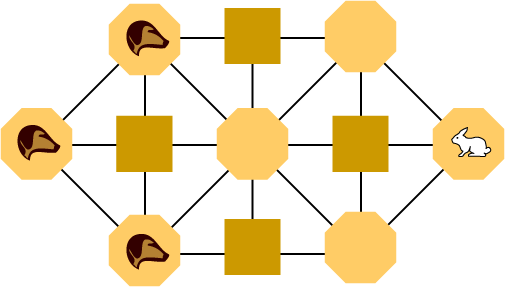
\includegraphics[width=300pt]{Hare_and_Hounds_board.png}
		\label{fig:Hare_and_Hounds_board}
	\end{figure}		
\end{frame}

\begin{frame}
    \frametitle{Rules of the game}
    \begin{itemize}
        \item Hounds win if hare cannot move
        \item Hare wins if it is to the left of the hounds
        \item Hounds can only move right, diagonally or vertically, one hound per turn
        \item Hare can move in any direction
        \item Players can only move to vacant spaces
    \end{itemize}
\end{frame}
%% Expectations (Rene)

\begin{frame}
    \frametitle{Expectations}
    \begin{itemize}
        \item Game is studied $\Rightarrow$ know expected outcome
        \item Perfect play $\Rightarrow$ hounds win
        \item Percentage of wins by hound is indication of performance
        \item Policy can also be evaluated
    \end{itemize}
\end{frame}
%% Differences in implementation (Xeryus)

% Method  (Xeryus)
%% Q learning
%% Experiments
\section{Method}
\begin{frame}
	\frametitle{Method}
	\begin{itemize}
		\item Q-learning
		\item Use annealing
	\end{itemize}
	\[ \hat{Q}(s_t, a_t) = \hat{Q}(s_t, a_t) + \eta \left(r_{t+1} + \gamma \max_{a_{t+1}} Q(s_{t+1}, a_{t+1}) - Q(s_t, a_t)\right) \]
\end{frame}

\begin{frame}
	\frametitle{Experimental setup}
	\begin{itemize}
		\item Train with varying $\gamma, \eta$ to build models
		\item Compare performance of different models
	\end{itemize}
\end{frame}

\section{Results}
% Results (Rene)
%% Statistics for parameters
\begin{frame}
    \frametitle{Results}
    \begin{itemize}
        \item Trained with 56 configurations
        \item Probability of hound wins as performance

            \phantom{M}

        \item Hare wins in beginning
        \item Hounds win at the end
    \end{itemize}
\end{frame}

\begin{frame}
    \frametitle{Results}
    \begin{itemize}
        \item Linear model
        \item Discount factor (gamma) significant ($p = 8.02 \times 10^-8$)
        \item Number of training significant ($p = 2.33 \times 10^-7$)
        \item Learning rate (eta) not significant ($p = 0.281$)
    \end{itemize}
\end{frame}

\begin{frame}
    \centering
    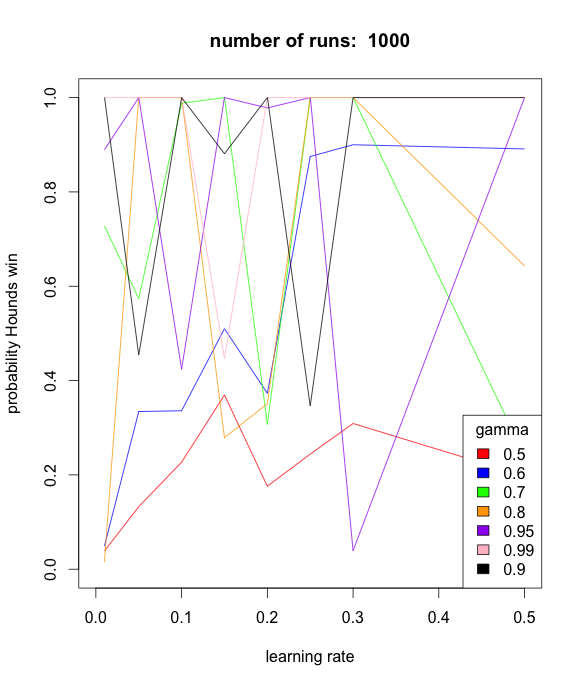
\includegraphics[width=0.65\textwidth]{r1000.png}
\end{frame}

\begin{frame}
    \centering
    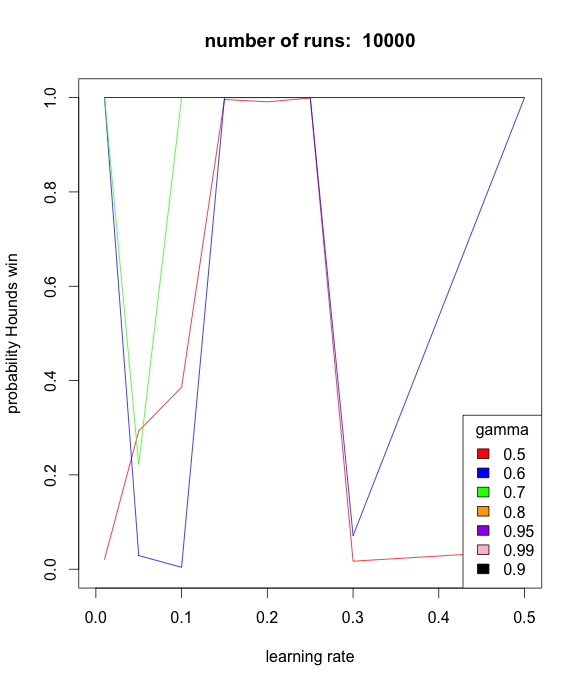
\includegraphics[width=0.65\textwidth]{r10000.png}
\end{frame}

\begin{frame}
    \centering
    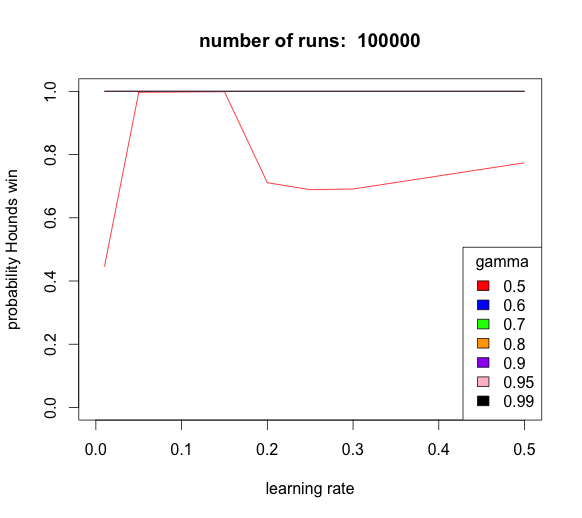
\includegraphics[width=0.65\textwidth]{r100000.png}
\end{frame}

%% Tie in with background

% Discussion (Siegrid)
%% Would longer training help?
%% How can we improve the system?
\begin{frame}
	\frametitle{Discussion}
	\begin{itemize}
		\item Would longer training change the outcome?
		\item Would other rules make the game more fair?
		\begin{itemize}[<+->]
        		\item<2-> Hounds may only move vertically 10 times in a row
	 		\item<3-> Hare wins with a tie
		\end{itemize}
	\end{itemize}
\end{frame}

\end{document}
